\begin{pastexam}[label={px:ncku-108-ee-ds-05}]{成大電機所 108 學年度 問答題第 4 題}
（問答）

Please show the postorder and the level-order traversal of the following tree. (10 points)

\begin{center}
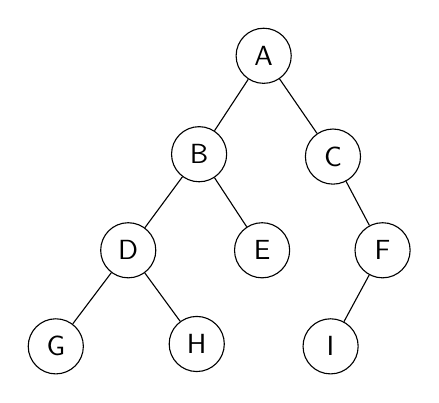
\begin{tikzpicture}[v/.style={circle,draw,minimum size=7mm,inner sep=0pt,font=\sffamily}]
\node[v] (A) at (11.02,-6.03) {A};
\node[v] (B) at (10.20,-7.28) {B};
\node[v] (C) at (11.90,-7.31) {C};
\node[v] (D) at (9.30,-8.50) {D};
\node[v] (E) at (11.00,-8.50) {E};
\node[v] (F) at (12.53,-8.50) {F};
\node[v] (G) at (8.38,-9.72) {G};
\node[v] (H) at (10.17,-9.69) {H};
\node[v] (I) at (11.87,-9.72) {I};
\draw (A) to (B);
\draw (A) to (C);
\draw (B) to (D);
\draw (B) to (E);
\draw (C) to (F);
\draw (D) to (G);
\draw (D) to (H);
\draw (F) to (I);
\end{tikzpicture}
\end{center}
\end{pastexam}

\begin{pastsoln}
先讀出樹的結構（看邊的方向）：A 的左、右子節點是 B、C；B 的左、右是 D、E；C 只有\textbf{右}子節點 F；
D 的左、右是 G、H；F 只有\textbf{左}子節點 I。 E、G、H、I 是葉節點。

\textbf{後序}（左子樹、右子樹、根，資結書第~7.3~節）：
\begin{itemize}
\item B 的子樹：D 的子樹是 G H D，接著 E，再 B：G H D E B。
\item C 的子樹：C 沒有左子樹；右子樹 F 的後序是 I F；再 C：I F C。
\item 最後是根 A。
\end{itemize}
\[
\text{後序：} G,\ H,\ D,\ E,\ B,\ I,\ F,\ C,\ A
\]

\textbf{層序}（從根開始一層一層、每層由左到右，用佇列，資結書第~7.3.2~節）：
\begin{center}
\small
\begin{tabular}{lll}
\toprule
取出 & 加入佇列 & 佇列（前 $\to$ 後） \\
\midrule
（開始） & A & A \\
A & B, C & B C \\
B & D, E & C D E \\
C & F & D E F \\
D & G, H & E F G H \\
E & & F G H \\
F & I & G H I \\
G、H、I & & （空） \\
\bottomrule
\end{tabular}
\end{center}
\[
\text{層序：} A,\ B,\ C,\ D,\ E,\ F,\ G,\ H,\ I
\]
第 1 層 A；第 2 層 B C；第 3 層 D E F；第 4 層 G H I。 I 雖然畫在 E 的下方附近，但它是 F 的子節點，在第 4 層的
最右邊。
\end{pastsoln}
